\documentclass{article}
\usepackage{cite}
\usepackage[margin=1in]{geometry}
\usepackage{amssymb}
\usepackage{mathtools}

\usepackage{amsthm}
\usepackage{amsmath}
\usepackage{slashed}
\usepackage{relsize}
\usepackage{threeparttable}
\usepackage{float}
\usepackage{booktabs}
\usepackage{boldline}
\usepackage{changepage}
\usepackage{physics}
\usepackage[inter-unit-product =\cdot]{siunitx}
\usepackage{setspace}

\usepackage[makeroom]{cancel}
\usepackage{pgfplots}

\usepackage{enumitem}
\usepackage{times}

\usepackage{tcolorbox}
\usepackage{mathrsfs}
\title{Optical Tweezers \\
\textsc{\normalsize Physics 443}}
\author{Kevin Evans}

\doublespacing

\begin{document}
	\maketitle
	\begin{abstract}
	\noindent Optical tweezers are a method of trapping small dielectric particles using highly-focused lasers. This paper introduces optical tweezers, giving a simplified description of its operation, then provides some historical background on its development. A derivation of its principles is discussed using a simplified description of Arthur Ashkin's early experiments. This derivation uses ray optics, finding a systems matrix. Then approximates the total gradient force as a function of distance from the beam axis. By plotting the gradient force, it becomes apparent how optical tweezers can trap particles within the beam axis. Next, an overview of using an objective lens within optical tweezers is provided. The addition of an objective provides stability when using a single beam laser and the resultant force equations are provided, but not derived.
	\end{abstract}
	
	\pagebreak
	
	\section{Introduction}
	Optical tweezers are a method of trapping small dielectric particles using highly-focused lasers. Optical tweezers use an incident Gaussian beam to create a force gradient perpendicular to the beam axis. The force gradient is due to incident light refracting across the dielectric bead and the emission of radiation pressure as it exits. For a unfocused beam, this creates an optical well in a single axis, bringing particles to the beam center but accelerating the particles along the axis in the direction of the light propagation. However, using multiple beams, a stable optical well is possible through several methods: including balancing the scattering force with gravity \cite{doi:10.1063/1.1653919} or opposing two lasers. Later developments have used a single convergent lens, allowing a single beam to create a stable optical well \cite{Ashkin:86}.
	
		
	These wells are capable of trapping particles on a microscopic scale. In early experiments, optical tweezers were demonstrated capable of non-invasively trapping and manipulating individual viruses and bacteria \cite{Ashkin1517}. Additionally, optical tweezers are capable of measuring miniscule piconewton forces. Optical tweezers have several applications in biology and has brought on a new field of single-molecule biophysics. 
	
	\section{Background}
	For over a century, it has been known that light can exert a pressure due to momentum carried by a photon. On the macro-level, this pressure is quite small; for the sun's radiation pressure, this is only the scale of several micropascals. On the molecular scale, this pressure can have noticeable effects.
	
	In the mid 1960s, At Bell Labs, Arthur Ashkin began development on an optical trap capable of trapping latex spheres suspended in water \cite{PhysRevLett.24.156}. Initially, this optical trap used a single Gaussian beam and would simultaneously trap particles along the beam axis and accelerate particles away from the light. Using two opposing beams would allow a ``true'' optical trap, bringing particles to a fixed location as the scattering forces are now balanced.
	
	In subsequent experiments, optical levitation was performed using a similar approach as the earlier optical trap. In these experiments, Ashkin uses a laser pointed upwards and balances the particle with the gravitational force \cite{doi:10.1063/1.1653919}. Another laser beam is used to trap a particle within the center of a chamber.
	
	By 1986, Ashkin began optically trapping \SI{10}{\um} to \SI{25}{\nm} particles using a single-beam gradient \cite{Ashkin:86}. In these experiments, the incident laser light is highly-convergent using a high NA microscope objective. This allows particles to be trapped within the additional gradient created by the objective's focus. In 2018---nearly 50 years after its invention---the Nobel Prize in Physics was awarded to Ashkin and his team for the development of optical tweezers. 
	
	\section{Theory of operation}
	In this section, two approaches are taken and discuss basic theory of the optical trap's operation. For the case of an unfocused laser, several assumptions are made to simplify the derivation and only an approximation of the gradient force is found. For the focused laser, the derivation is fairly rigorous\footnote{And I don't fully understand how parts of the forces are derived.}, so only qualitative outline of its theory is provided, as well as the results found by Ashkin.
	
	\subsection{Unfocused Laser}
	A simplification of Ashkin's early optical trap using a single Gaussian beam without an objective lens can be described using ray diagrams and ray-transfer matrices. To simplify the derivation, several assumptions have been made: (1) the surrounding medium has an index of refraction of $1$, (2) there are no external forces, (3) the beam source has an unfocused Gaussian profile, (4) the scattering forces due to reflection are ignored. An optical trap is shown in Figure \ref{fig:lens} with a single Gaussian beam. Here, two paths $A$ and $B$ are drawn with different incident intensities specified by a Gaussian source and depicted by the thicknesses of each line. As the light refracts and exits the sphere, each ray imparts radiation pressure proportional to the incident light, resulting in a net gradient force toward the center axis of the Gaussian beam.
	
	\begin{figure}[H]
		\begin{center}
			\includegraphics[width=0.7\linewidth]{lens}
		\end{center}
		\caption{Diagram of a particle in an incident Gaussian beam. Note the axial gradient and scattering pressure component axes.}
		\label{fig:lens}
	\end{figure}
	
	\pagebreak
	
	If we again consider the sphere of radius $R$ in air with index of refraction $n$, it can be characterized by a systems matrix $\mathbf{M}$---including two refraction matrices ($\mathbb{R}$) and one translation matrix ($\mathbb{T}$), \begin{align*}
		\mathbf{M} & = \mathbb{R}_2 \; \mathbb{T} \; \mathbb{R}_1 \\
			& = \begin{pmatrix}
				1 & 0 \\
				-\frac{n - 1}{R} & n
			\end{pmatrix}
			\begin{pmatrix}
				1 & 2R \\
				0 & 1
			\end{pmatrix}
			\begin{pmatrix}
				1 & 0 \\
				\frac{1 - n}{nR} & \frac{1}{n}
			\end{pmatrix} \\
			& = \begin{pmatrix}
				\frac{2(1-n)}{n} + 1 & \frac{2R}{n} \\
				\frac{2(1-n)}{nR} & \frac{2(1-n)}{n} + 1
			\end{pmatrix}
	\end{align*}
	From the systems matrix, and as the incident angle is assumed to be zero relative to the lens axis, the light exits with angle $\gamma'$, \begin{align}
		\gamma'(x) & = \frac{2(1-n)}{nR} x \label{eq:gamma}
	\end{align}
	where $x$ is the distance from the center axis of the lens.
	
	For a TEM$_{00}$ beam, its intensity is given proportional to a Gaussian distribution and is simplified\footnote{I've chosen to omit the waist radius $w_0$ and assume straight, parallel incident rays for simplicity's sake and will instead use $\alpha$ to describe the beam width.} here as \begin{align*}
		I_G(r) & = I_0 \exp(-\alpha r^2)
	\end{align*}
	with $r$ as the distance from the beam center, $\alpha$ as an arbitrary positive constant, and $I_0$ as the maximum center intensity.
	
	For the gradient pressure, i.e. the pressure along the vertical axis of Figure \ref{fig:lens}, it can be found using intensity at the angle given by \eqref{eq:gamma}. The radiation force is proportional to the emission intensity as \begin{align*}
		F_\mathrm{e} & \propto \frac{ I_e }{c}
	\end{align*}
	Here, the emission intensity at $r$ in the vertical direction is found as \begin{align*}
		I_e (r) & = I_G(r) \sin[\gamma'(-r + d)] %%%% TODO check if this makes sense
	\end{align*}
	where $d$ is the particle's distance from the center of the beam.
	The total gradient force can be calculated as a function of distance from the beam axis $d$, \begin{align*}
		F_e(d) & \propto \frac{1}{c}\int_{d - R}^{d + R} I(r) \dd{r} \\
			& \propto \frac{ I_0 }{c} \int_{d - R}^{d+R} \exp(-\alpha r^2) \sin\left[ \frac{2(1-n)}{nR} (-r + d) \right] \dd{r}
	\end{align*}
	After taking the paraxial approximation before integrating for the sine\footnote{I'm actually not sure if this is valid here. }, the approximate emitted pressure as a function of the distance from the Gaussian center is given by a hyperbolic sinusoid \begin{align*}
		F_e(d) & \propto \frac{I_0 (n-1)}{\alpha n c R} \left(e^{-\alpha(d-R)^2} - e^{-\alpha(d+R)^2}\right)
	\end{align*}
	Plotting this in Figure \ref{fig:plot} with arbitrary units, the restorative gradient force becomes evident. If the particle is below the center of the light beam, it will have a emit a positive radiation pressure, bringing the particle closer to the center. Similarly, if the particle is above the center, it will emit a negative pressure until the particle reaches the inflection point at the center of the beam.
		
	\begin{figure}[H]
		\centering
		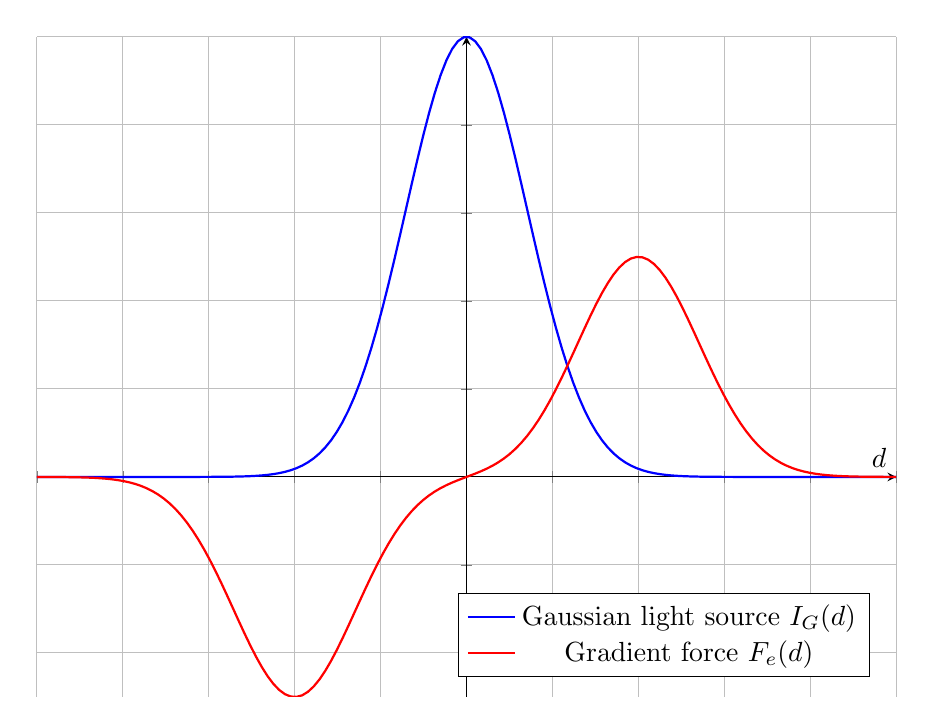
\begin{tikzpicture}
			\begin{axis}[
				scale only axis,
				width=0.9\linewidth,
				height=0.3\paperheight,
				yticklabels={,,},
				xticklabels={,,},
				grid=both,
				clip,
				ymax=1,
				xlabel=$d$,
				ylabel={},
				samples=150,
				no markers,
				axis lines=center,
				legend pos=south east
				]
				% use TeX as calculator:
				\addplot[thick,blue]{e^(-x^2)};
				\addplot[thick,red]{1/2 * (e^(-(x-2)^2) - e^(-(x+2)^2))};
%				\addplot[thick,green]{x*e^(-x^2)};
				\addlegendentry{Gaussian light source $I_G(d)$}
				\addlegendentry{Gradient force $F_e(d)$}
			\end{axis}
		\end{tikzpicture}
		\caption{The incident light and resultant restorative forces.}
		\label{fig:plot}
	\end{figure}

	In the derivation, the scattering force was ignored and only the gradient force was approximated. For a single laser beam, there is an additional scattering force along the direction of the beam, i.e. from the cosine component of the pressure. This force can be balanced using a second laser of equal qualities in the opposite direction of the beam. In Askin's 1969 experiment, equal lasers are placed opposite of one another, and the particle is trapped directly between\cite{PhysRevLett.24.156}. This prevents scattering acceleration in the direction of the wave. Alternatively, the beam can be placed such that the light is pointed upward against the gravitational force. In doing so, optical levitation is possible though has several limitations \cite{doi:10.1063/1.1653919}. This type of trap required a single beam and could support \SI{20}{\um} glass beads using \SI{250}{\mW} lasers.

	\subsection{Single lens optical trap}
	In subsequent experiments, Ashkin began using a high-NA objective lens to focus the incident beam. A diagram of this optical trap is shown in Figure \ref{fig:opticaltrapfocused}. In Figure \ref{fig:opticaltrapfocused}(a) the bead is located under the focus of the beam. As Ray 1 refracts and exits across the bead, the light undergoes a change in momentum. As a result, the particles must undergo an equal and opposite change in momentum, shown by $F_1$ in the diagram. For all incident rays on the bead, the resultant force $F_\mathrm{net}$ is upward toward the beam focus. Similarly, in Figure \ref{fig:opticaltrapfocused}(b), the change in momentum results in a net downward force toward the focus of the beam. In both scenarios, the bead has an upward force component due to the reflection. This results in a higher force in Figure \ref{fig:opticaltrapfocused}(a) than (b).
	
	
	\begin{figure}
		\centering
		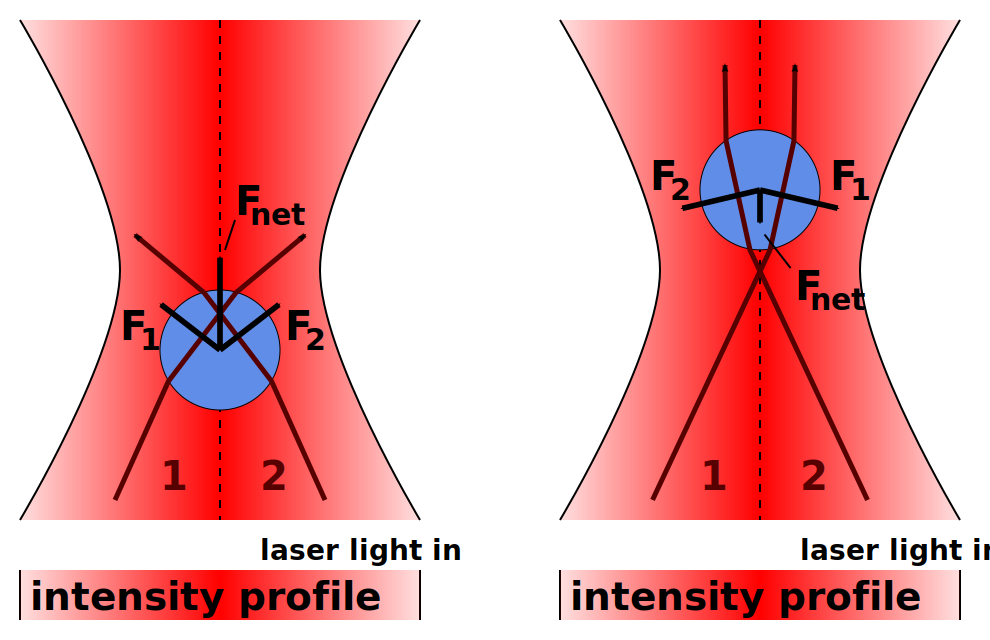
\includegraphics[width=0.7\linewidth]{Optical_trap_focused}
		\\
		(a) \hspace{16.4em} (b)
		
		\caption{{Forces on a dielectric bead using a focused laser beam, (a) the particle below the focus on the beam axis, (b) the particle above the focus. \\ {\small Source: Roland Koebler, 2011. Licensed under CC BY 3.0.}}}
		\label{fig:opticaltrapfocused}
	\end{figure}
	
	To calculate the forces, we can again divide the force into two components: the scattering force and the gradient force. It can be shown\cite{Ashkin:86} for a particle in a medium of $n_b$ and polarizability $\alpha$, the forces \begin{align*}
		F_\mathrm{scatt} & = \frac{I_0}{c} \frac{128 \pi^5 r^6}{3 \lambda^4} \left(\frac{m^2 - 1}{m^2+2}\right) n_b \\
		F_\mathrm{grad} & = -\frac{n_b}{2} \alpha \grad{E^2} = -\frac{n_b^3 r^3}{2} \left(\frac{m^2 - 1}{m^2 -2}\right) \grad{E^2}
	\end{align*}
	where $I_0$ is the intensity and $m$ is the effective index. 
	
	Once a particle is trapped, it will remain in the focus of the laser indefinitely. If the particle exerts a force or has an external force exerted on it, it can overcome the gradient force. In this instance, the intensity of the laser can be increased until the particle remains at equilibrium, and the change in the intensity can be used to calculate the minuscule forces.

	
	
	
	\pagebreak
	
	\bibliography{refs}{}
	\bibliographystyle{plain}
	
\end{document}